\documentclass[a4paper, 12pt]{article}
\usepackage[utf8]{inputenc}
\usepackage{enumitem}
\usepackage{graphicx}
\usepackage{float}
\usepackage{polski}
\usepackage{subfig}
\usepackage{hyperref}
\usepackage{mathtools}
\usepackage{listings}
\usepackage{mathalfa}

\title{Softcomputing}
\author{Bogusław Matysik, Paweł Zaborowski}
\date{15th January 2020}

%http://www.zsk.ict.pwr.wroc.pl/zsk/repository/dydaktyka/sip/softcomputing/softcomputing_5.pdf
\begin{document}

\begin{titlepage}
    \makeatletter
    \vspace{1cm}
    \begin{center}
        
\includegraphics[width=0.75\textwidth]{PWr-logo_ang.png} \par
        \vspace{0.2cm}
        \Large Faculty Of Electronics \par
        \vspace{1.25cm}
        {    
            \bfseries
            Computer Science \\
            \vspace{0.25cm}
    	    \normalsize Internet Engineering \par
    	    \vspace{2cm}
    	    \Huge \@title \\
    	}
    	\vspace{0.5cm}
        \large Genetic Algorithms for maxima search of multimodal functions
    \end{center}
    \null
    \vfill
    \begin{flushright}
        Authors: \\
        Bogusław Matysik \\
        Paweł Zaborowski \\
    \end{flushright}
    \vspace{0.5cm}
\end{titlepage}

\newpage
\tableofcontents

\newpage
\section{Introduction}

\subsection{Function}

In our project we chosen two different functions. One more complex than the second one. We compared accuracy of the results of the both of them. They are more wisely described in the next sections. Both of these functions were tested on the same variables' restrictions.
It is worth mentioning that genetic algorithm is heuristic algorithm. We cannot be sure about the result since they are not perfectly exact. Every time it is some kind of estimation.
	

\section{Theory}

\subsection{Genetic algorithm in general}

Common characteristic of evolution algorithm which distinguish them from other traditional optimization methods are:	
\begin{itemize}
	\item usage of the genetic operators that are adapted to the form of solutions
	\item processing a population of solutions leading to a parallel search of solution spaces from different points
	\item quality of current solutions is enough to direct solution process in proper way
	\item purposeful introduction of random elements
\end{itemize}

Algorithm process:

\begin{center}
	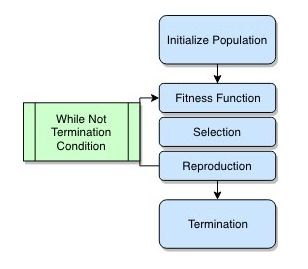
\includegraphics[width=0.8\textwidth]{alg_loop.png} 
\end{center}

The most commonly used chromosome coding:
\begin{itemize}
	\item a vector of genes each of which can be a single or multi-bit integer or a real number
	\item using tree data structures
\end{itemize}

For each population we need to calculate probability of being selected p:

	\[  p_s = \dfrac{f(x)}{\sum{f(x)}}\]
		

Chromosomes with the best value of fitness function have greater chance to be chosen.

Methods of selection:

\begin{itemize}
	\item Roulette wheel method 
	\item Ranking list
	\item Tournament 

\end{itemize}

%Reproduction–new population creation using the selected set of parents
%crossover–mutation 
%new population–new created chromosomes are the new population –new set of chromosomes -parents

Crossing's aim is to concatenate, in different combinations, characteristics coming from different individuals from population. "Child" has set of characteristics that are combination of parents' characteristics.

Mutation is about increasing variety of individuals. It introduces to genotype random changes. In that way we can protect of premature convergence of the algorithm.



Crossover operation


\section{Implementation}

In this paragraph we described each of the stage of our implementation of genetic algorithm. 
We tested our results with different amount of initial population size and most of all iterations of algorithm.
At the begging we started with initial population size equals 100 and 100 of iterations.

The algorithm begins by initializing a population of individuals using default values. Then, it runs each member of that population through a fitness function. After that it selects the fittest members of the population to reproduce using a method defined in the reproduction function. The evaluation and reproduction is repeated until a desired number of iterations have passed. At end, the algorithm presents the best member or members of the population according to the fitness function.

\subsection{Fitness function}

We prepared two functions:
\begin{enumerate}
	\item \[20*x^2 + y^2 - 10*(cos(2 * \pi * x) + sin(2 * \pi * y) \] \\
	\item \[sin(3*x) * cos(3*y) / 10\]
\end{enumerate}

The variable restriction for both of them is set to $<$-1;1$>$.
The aim is to maximize them, so found best input.

\subsection{Selection function}

The selection function takes the population and the results of the fitness function to determine who should reproduce in the next iteration. The selection function calculates a threshold from scores from fitness function. For example, it may calculate the average score and only keep the top half of the population as in our case, because we want to find maximum value. It passes the selected population and average score into the reproduction function and deletes the rejected individuals. 

\begin{center}
	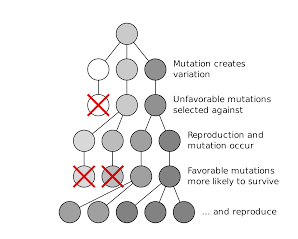
\includegraphics[width=0.8\textwidth]{sel_function.png} 
\end{center}


\begin{lstlisting}
def evaluate_generation(population):
	scores = []
	total = 0
	for individual in population:
		r = fitness_function(individual[0], individual[1])
		scores.append(r)
		total += r
	else:
		print("error: Wrong number of arguments received")
	avg = total / len(scores)
	return scores, avg
\end{lstlisting}

indivudal[] is two item array because we have two variables in our fitness function.

\subsection{Reproduction function}

The reproduction function determines how to expand the population based on the existing members. Modifying the behavior and hyperparameters of the reproduction function.
The simplest reproduction method is mutation, where each new member is based on a single individual and this is the method we used in out algorithm.

Besides that, crossover is a more complex method of reproduction, where each new individual is based on some combination of existing individuals. Crossover still mutates the new organism’s attributes, but does so by applying a function of multiple organisms’ attributes.

In our process we decided to confine just with mutation method. \\

\begin{lstlisting}
def mutate(individual):
	new = []
	for attribute in individual:
		new.append(attribute + 
			random.normalvariate(0, attribute + .1))  # Random factor of normal distribution
	return new
\end{lstlisting} 

It modifies each attribute of an individual by a random factor. In particular, we use a normal variate distribution that has a higher probability of a smaller modification as it has a mean near zero. When creating new individuals, it is important to consider how different they should be from the parents. If the difference is too small, the algorithm will require many iterations to reach a max, but if the difference is too big, the output will be imprecise and may miss the maximum.


\subsection{Termination function}

After all of the iterations have run, the termination function takes the final population and evaluates it on the fitness function to return the best individual(score). In this case, the best individual is the estimated maximum value of the function and its attributes are the estimated optimal inputs to given function. The inputs may be greater or less than the actual best inputs, but the estimated maximum value will by definition be less than or equal to the true global maximum.

\begin{lstlisting}
def find_best(population):
	best = None
	val = None
	for individual in population:
		r = fitness_function(individual[0], individual[1])
		try:
			if r > val:
				best = individual
				val = r
		except:
			best = individual
			val = r
	return best, val
\end{lstlisting}


Running the simpler function on 100 individuals with 100 iterations got us within one thousand of the best answer almost instantly.

\subsection{Technology}

Technologies we used to implement algorithm:
\begin{itemize}
	\item python 3.6
	\item libraries: numpy, math, matplotlib, mpl\_toolkits
\end{itemize}

To compare out results we used WolframAlpha tool. 

\section{Experiments}

\subsection{First function}

 \[20*x^2 + y^2 - 10*(cos(2 * \pi * x) + sin(2 * \pi * y) \] 

%100 iterations on a population of 100
%The optimal input is [5.847e+90, -0.1] with a value of 6.838e+182

%150 iterations on a population of 100
%The optimal input is [-2.232e+126, -0.1] with a value of 9.971e+253

%170 iterations on a population of 100
%The optimal input is [8.163e+138, -0.1] with a value of 1.332e+279

%100 iterations on a population of 120
%The optimal input is [-9.071e+92, -0.1] with a value of 1.646e+187

%100 iterations on a population of 150
%The optimal input is [3.074e+97, -0.1] with a value of 1.890e+196

%150 iterations on a population of 150
%The optimal input is [-4.447e+140, -0.1] with a value of 3.955e+282

	\begin{table}[!h]
	\begin{tabular}{lllll}
		population: 100 &                                                                         &  &  &  \\
		100      & The optimal input is [5.847e+90, -0.1] with a value of 6.838e+182
		   &  &  &  \\
		150      & The optimal input is [-2.232e+126, -0.1] with a value of 9.971e+253
		 &  &  &  \\
		170      & The optimal input is [8.163e+138, -0.1] with a value of 1.332e+279  &  &  & 
	\end{tabular}
\end{table}

\begin{table}[!h]
	\begin{tabular}{lllll}
		population: 120 &                                                                         &  &  &  \\
		100      &    &  &  &  \\
		150      & The optimal input is [-9.071e+92, -0.1] with a value of 1.646e+187 &  &  &  \\
		170      &   &  &  & 
	\end{tabular}
\end{table}

\begin{table}[!h]
	\begin{tabular}{lllll}
		population: 150 &                                                                         &  &  &  \\
		100      & The optimal input is [3.074e+97, -0.1] with a value of 1.890e+196   &  &  &  \\
		150      & The optimal input is [-4.447e+140, -0.1] with a value of 3.955e+282 &  &  &  \\
		170      &  &  &  & 
	\end{tabular}
\end{table}

the bigger population the bigger scores to choose.

\subsection{Second function}

 \[sin(3*x) * cos(3*y) / 10\]
 
 %100 iterations on a population of 100
 %The optimal input is [0.541, 0.012] with a value of 0.333
 %100 iterations on a population of 120
 %The optimal input is [0.524, 0.002] with a value of 0.333
 %100 iterations on a population of 150
 %The optimal input is [0.516, -0.014] with a value of 0.333
 
 %150 iterations on a population of 100
 %The optimal input is [0.537, 0.002] with a value of 0.333
 %150 iterations on a population of 150
 %The optimal input is [0.512, 0.006] with a value of 0.333
 
 %170 iterations on a population of 100
 %The optimal input is [0.513, -0.012] with a value of 0.333
 %170 iterations on a population of 150
 %The optimal input is [0.527, 0.001] with a value of 0.333
 
 \begin{table}[!h]
 	\begin{tabular}{lllll}
 		population: 100 &                                                                         &  &  &  \\
 		100      & The optimal input is [0.541, 0.012] with a value of 0.333
 		&  &  &  \\
 		150      &  The optimal input is [0.537, 0.002] with a value of 0.333
 		&  &  &  \\
 		170      & The optimal input is [0.513, -0.012] with a value of 0.333  &  &  & 
 	\end{tabular}
 \end{table}
 
 \begin{table}[!h]
 	\begin{tabular}{lllll}
 		population: 120 &                                                                         &  &  &  \\
 		100      &  The optimal input is [0.524, 0.002] with a value of 0.333  &  &  &  \\
 		150      & The optimal input is [0.512, 0.006] with a value of 0.333 &  &  &  \\
 		170      &   &  &  & 
 	\end{tabular}
 \end{table}
\newpage
 
 \begin{table}[!h]
 	\begin{tabular}{lllll}
 		population: 150 &                                                                         &  &  &  \\
 		100      & The optimal input is [0.512, 0.006] with a value of 0.333    &  &  &  \\
 		150      &  The optimal input is [0.516, -0.014] with a value of 0.333 &  &  &  \\
 		170      &  The optimal input is [0.527, 0.001] with a value of 0.333 &  &  & 
 	\end{tabular}
 \end{table}


\section{Plots}

\subsection{First function} 

\[20*x^2 + y^2 - 10*(cos(2 * \pi * x) + sin(2 * \pi * y) \]

\begin{center}
	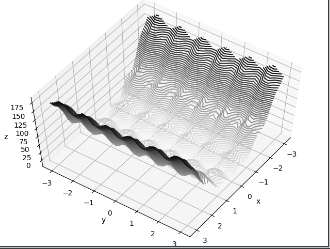
\includegraphics[width=0.8\textwidth]{fit_fun.png} \par
\end{center}

\newpage
\subsection{Second function}

\[sin(3*x) * cos(3*y) / 10\]

\begin{center}
	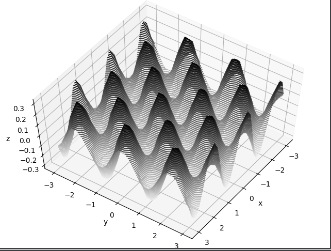
\includegraphics[width=0.8\textwidth]{sec_fun.png} \par
\end{center}


\section{Results \& conclusions}

 %   min_loc = opt.fmin(lambda vec: -fitness_function(vec[0], vec[1]), [-1.0, 1.0])
To compare our results with the correct ones we used scipy.optimize library. In scipy.optimize.fmin() function we put our function in parameter, with two variables and then negate it we get maximum: 
\begin{lstlisting}
max = opt.fmin(lambda vec: -fitness_function(vec[0], vec[1]), [-1.0, 1.0])
\end{lstlisting}
This lib uses the downhill simplex algorithm.

Results:
\begin{itemize}
	\item function 1): \\  Current function value: 0.333333 \\ $[$-0.52363581,  1.04718372$]$
	\item function 2): 	\\  Current function value: 0.333333 \\ $[$-0.52363581,  1.04718372$]$
		
\end{itemize}
\end{document}